% ============================================================================
% Networks Decide for Us — EUSN 2026 (European Conference on Social Networks)
% Simplified two-network arc (CPIN architecture, SNA language):
%   Result 1: adoption maps · Result 2: the structural premium (+ channel split)
%   Result 3: the shape of change (tipping cut; no exponents in main deck)
% GSS-SH and the physics mapping live in BACKUP slides (Q&A ammunition).
% Baseline label: "Randomized" (same people, same size & density) — neutral on
% the ER vs degree-preserving question (see checks-claude notes, 2026-08-12).
% Style replicates the CPIN / SUNBELT / "JORNADA REDES" deck.
% Compile: pdflatex presentation-eusn26.tex  (run twice)
% ============================================================================
\documentclass[aspectratio=169,11pt]{beamer}

\usepackage[utf8]{inputenc}
\usepackage[T1]{fontenc}
\usepackage{amsmath, amssymb}
\usepackage{graphicx}
\usepackage{booktabs}
\usepackage{array}
\usepackage{xcolor}
\usepackage{colortbl}   % \rowcolor in tables
\usepackage{tikz}
\usepackage{qrcode}
\usetikzlibrary{arrows.meta, positioning, calc, decorations.pathreplacing}

% ---------- Fonts: clean humanist sans, professional math ----------
\usefonttheme{professionalfonts}
\usepackage{helvet}
\renewcommand{\familydefault}{\sfdefault}

% ---------- Colors (matched to the JORNADA deck) ----------
\definecolor{ndred}{RGB}{222,32,38}       % bright red rule
\definecolor{ndreddark}{RGB}{176,22,28}   % darker brick red (subtitles)
\definecolor{ndgreen}{RGB}{0,118,54}      % green reference markers (darker)
\definecolor{ndblue}{RGB}{30,90,200}      % accent blue
\definecolor{ndgray}{RGB}{90,90,90}

% ---------- Strip all Beamer chrome ----------
\setbeamertemplate{navigation symbols}{}
\setbeamercolor{normal text}{fg=black,bg=white}
\setbeamercolor{structure}{fg=ndreddark}
\setbeamertemplate{itemize item}{\color{ndreddark}\textbullet}
\setbeamertemplate{itemize subitem}{\color{ndgray}\textendash}

% ---------- Frame title: centered black title + full-width red rule ----------
\setbeamercolor{frametitle}{fg=black,bg=white}
\setbeamerfont{frametitle}{size=\Large, series=\mdseries}
\setbeamertemplate{frametitle}{%
  \vspace{0.35cm}%
  \begin{center}\insertframetitle\end{center}%
  \vspace{-0.18cm}%
  {\color{ndred}\hrule height 1.1pt}%
}

% ---------- Minimal footline: page number only ----------
\setbeamertemplate{footline}{%
  \hfill{\color{ndgray}\scriptsize\insertframenumber}\hspace{0.5cm}\vspace{0.2cm}}

% ---------- Helper macros ----------
\newcommand{\refn}[1]{{\color{ndgreen}[#1]}}
\newcommand{\emphr}[1]{{\color{ndreddark}\textbf{#1}}}

% Section-divider slide
\newcommand{\sectionslide}[1]{%
  \begin{frame}[plain]
    \vfill
    \begin{center}
      {\Large #1}\\[2pt]
      {\color{ndred}\rule{0.30\textwidth}{1.1pt}}
    \end{center}
    \vfill
  \end{frame}}

% ============================================================================
\title{Networks Decide for Us}
\subtitle{The Emergence of Adoption in Homophily-Imputed Social Topologies}
\author{Aníbal Olivera M.}
\date{}

\begin{document}

% ---------------------------------------------------------------- 1. TITLE
\begin{frame}[plain]
  \vspace{0.5cm}
  \begin{center}
    
\includegraphics[height=1.0cm]{UDD.png}\hspace{1.2cm}\raisebox{0.25cm}{
\includegraphics[height=0.5cm]{poliCICS.pdf}}
  \end{center}
  \vspace{0.9cm}
  \begin{center}
    {\LARGE \textbf{Networks Decide for Us}}\\[0.5cm]
    {\large \color{ndreddark} The Emergence of Adoption in Homophily-Imputed Social Topologies}
  \end{center}
  \vspace{1.2cm}
  \begin{center}
    {\normalsize Aníbal Olivera M.}\\[2pt]
    {\footnotesize PhD(c) in Social Complexity Sciences, (UDD, CICS)}\\[2pt]
    {\footnotesize with Jorge Fábrega (UDD, CICS)}
  \end{center}
  \vfill
  \begin{center}
    {\scriptsize\color{ndgray} EUSN 2026 — European Conference on Social Networks}
  \end{center}
\end{frame}

% ---------------------------------------------------------------- 2. THE QUESTION
\begin{frame}{The question}
\begin{itemize}
  \item Collective behaviors — innovations, mobilizations — spread as
        \emphr{adoption cascades} on social networks.
  \vspace{0.25cm}
  \item We can measure \emphr{who people are} (preferences, from surveys), and we
        know \emphr{how they cluster} (multidimensional homophily) \refn{1,2}.
  \item Models usually run on synthetic networks,
        with invented preferences.
  \vspace{0.25cm}
  \item Our experiment: \emphr{fix the real people}, and rewire the ties.
\end{itemize}
\vspace{0.35cm}
\begin{center}
\fcolorbox{ndred}{white}{\parbox{0.92\textwidth}{\centering
Conditional on \emph{fixed individual preferences}, to what extent does the\\
\emphr{empirical network structure} — shaped by homophily —\\
govern the diffusion of collective behaviors?}}
\end{center}
\end{frame}

% ================================================================ THE MODEL
\sectionslide{The model}

% ---- 3. Rational choice (copied from SUNBELT deck)
\begin{frame}{Adoption, part 1 — Rational Choice}
\begin{itemize}
  \item A behavior has an \emph{Intrinsic Utility Level} \emphr{IUL}, $\Gamma\in[0,1]$.
  \item Each person has a \emph{Minimum Utility Requirement} \emphr{MUR}, $q_i\in[0,1]$,
        representing their aversion to adopting the behavior.
\end{itemize}
\vspace{0.1cm}
\begin{center}
An agent adopts on its own iff\quad
\fcolorbox{ndred}{white}{$\;q_i \le \Gamma \;\implies\; a_i = 1\;$}
\end{center}
\vspace{0.15cm}
\begin{center}
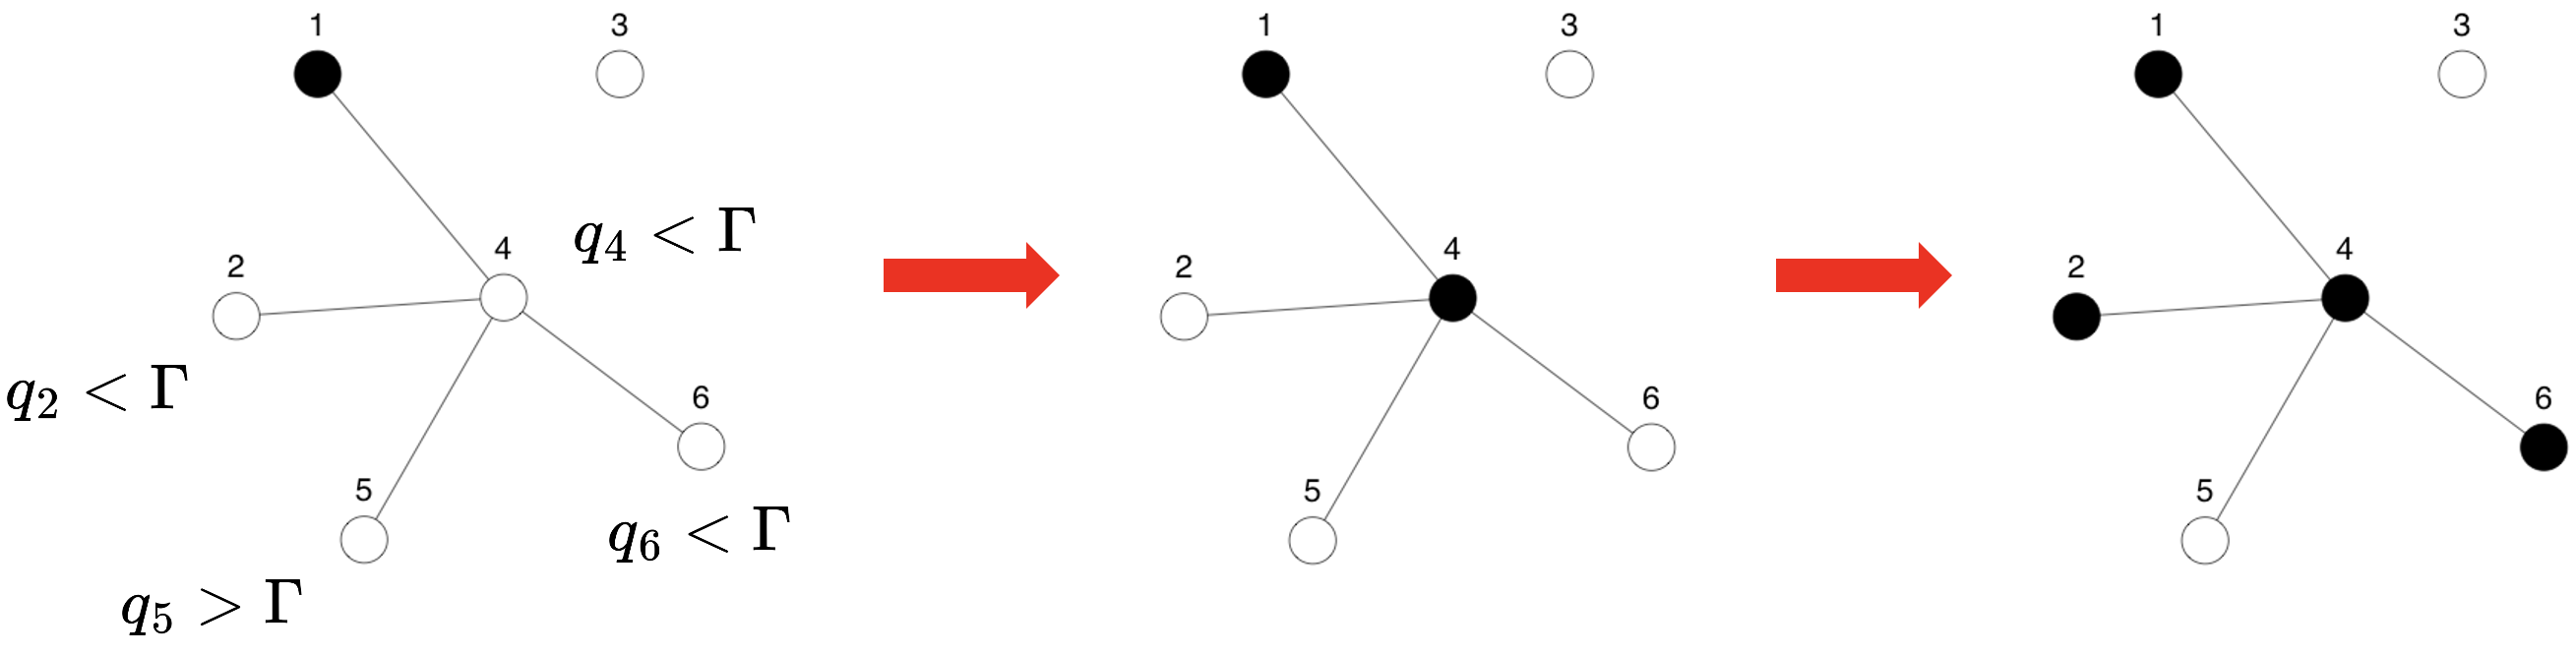
\includegraphics[width=0.95\textwidth]{graph-rational-choice.png}
\end{center}
\end{frame}

% ---- 4. Selective social influence (copied from SUNBELT deck)
\begin{frame}{Adoption, part 2 — Selective Social Influence}
Adopt by peer contagion if $\tau_i \le \tilde{E}_i$ \refn{3}
— but only those socially \emph{close} count \refn{4}:
\vspace{0.05cm}
\begin{equation*}
  \tilde{E}_i \equiv \frac{\sum_{j\neq i}\mathbf{X}_{ij}\,\tilde{a}_j}{\sum_{j\neq i}\mathbf{X}_{ij}},
  \qquad
  \tilde{a}_j = 1 \iff a_j = 1 \;\wedge\; U_{ij} \le \sigma\!\left(MSP - d_{ij}\right)
\end{equation*}
\begin{itemize}
  \item There is a Maximum Social Proximity \emphr{MSP} where the limit of influence sits.
\end{itemize}
\vspace{0.05cm}
\begin{center}
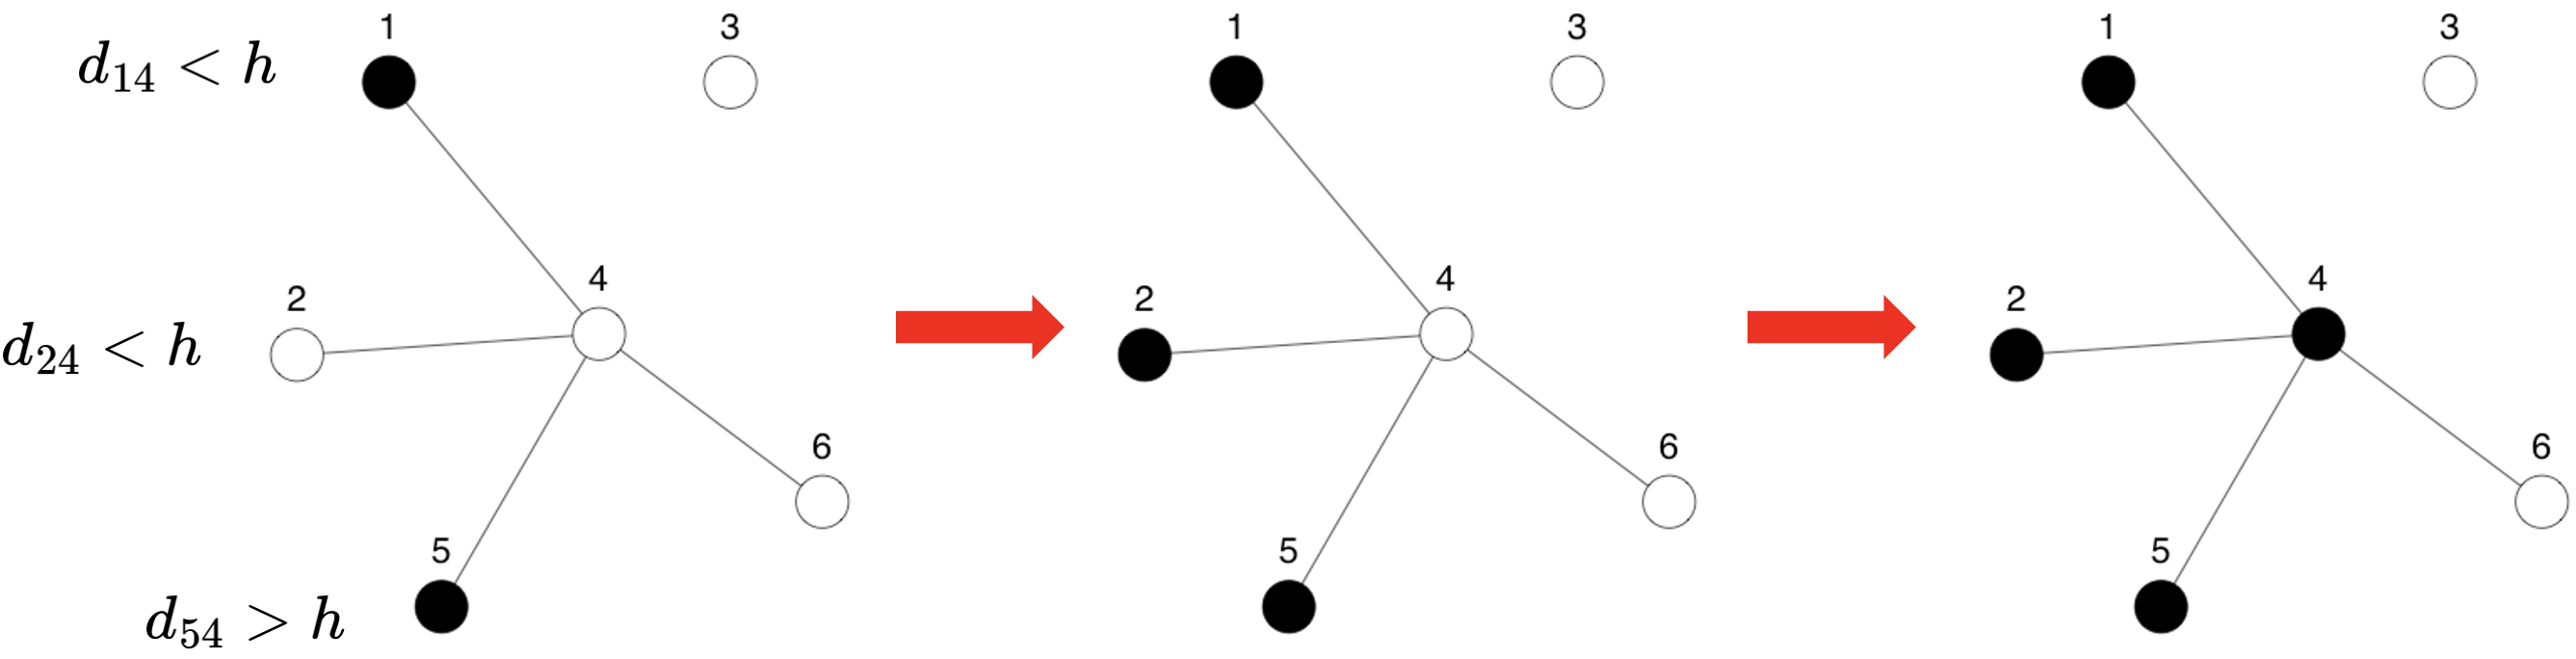
\includegraphics[width=0.9\textwidth]{graph-social-influence.png}
\end{center}
\end{frame}

% ================================================================ PIPELINE
\sectionslide{Imputing structure \& running the model}

% ---- 5. THE PIPELINE (copied from SUNBELT deck)
\begin{frame}{Imputing a network onto a survey}
\begin{center}
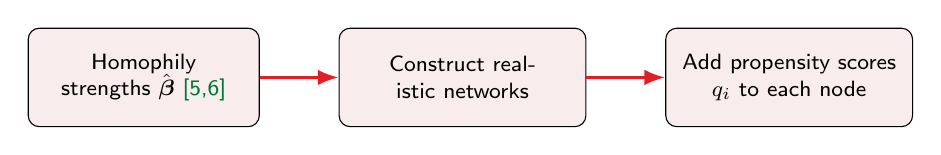
\begin{tikzpicture}[every node/.style={font=\footnotesize}]
  \node[draw,rounded corners,fill=ndreddark!8,text width=2.7cm,align=center,
        minimum height=1.25cm] (a) {Homophily strengths $\hat{\boldsymbol{\beta}}$ \refn{5,6}};
  \node[draw,rounded corners,fill=ndreddark!8,text width=2.9cm,align=center,
        minimum height=1.25cm,right=1.0cm of a] (b) {Construct realistic networks};
  \node[draw,rounded corners,fill=ndreddark!8,text width=2.9cm,align=center,
        minimum height=1.25cm,right=1.0cm of b] (c) {Add propensity scores $q_i$ to each node};
  \draw[-{Latex},ndred,line width=1pt] (a)--(b);
  \draw[-{Latex},ndred,line width=1pt] (b)--(c);
\end{tikzpicture}
\end{center}
\vspace{0.2cm}
\begin{columns}[c]
\column{0.52\textwidth}
\footnotesize
Tie probability is a function of social distance (age, sex, education, race, religion):
\vspace{0.2cm}
\begin{equation*}
  \mathrm{logit}\,\Pr(Y_{ij}=1)=\alpha+\boldsymbol\beta^\top \mathbf{d}_{ij}
\end{equation*}

$\hat{\boldsymbol\beta}$ comes from GSS confidant data \refn{5}; propensities $q_i$ come from
real survey answers (innovation, collective action).
\column{0.48\textwidth}
\centering
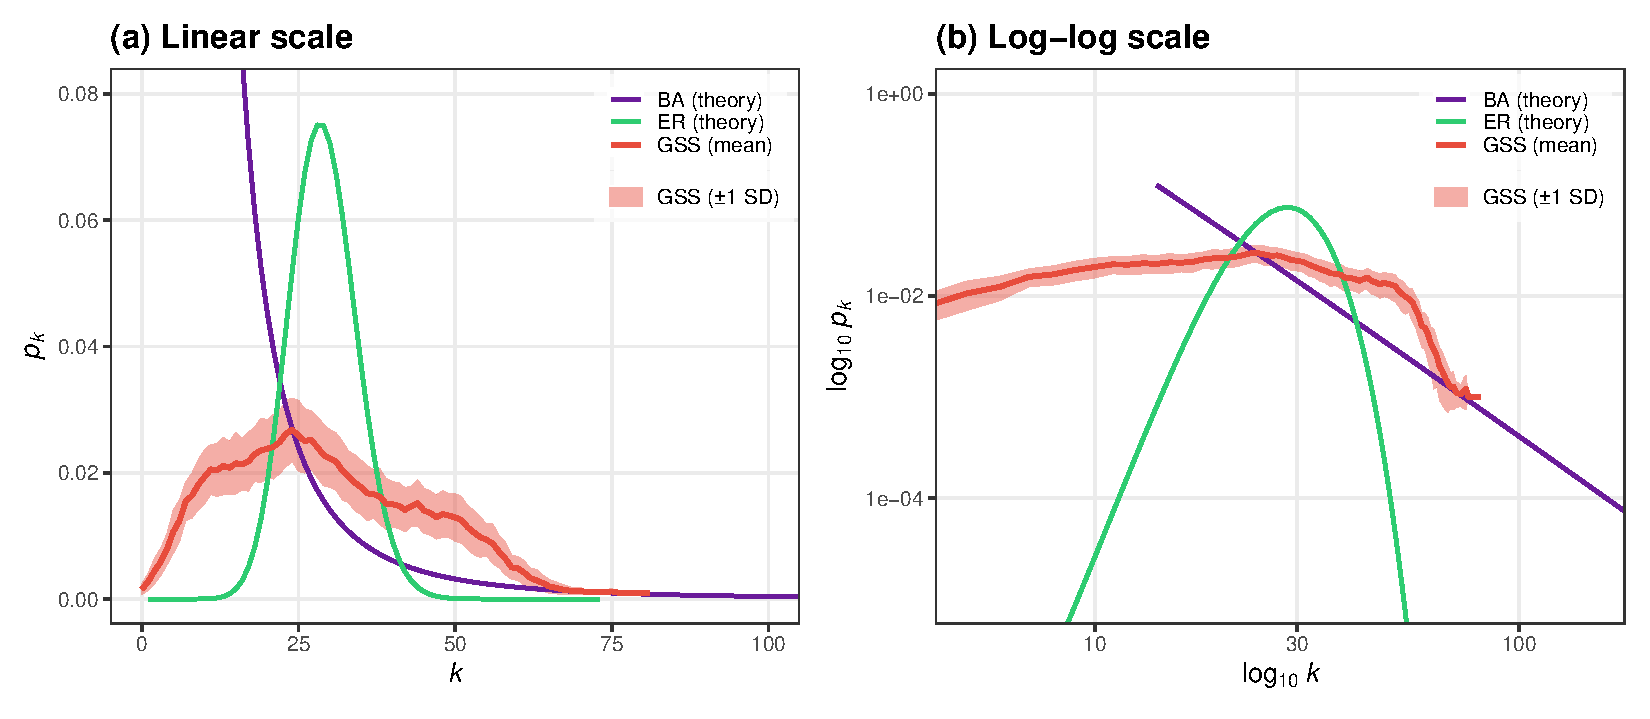
\includegraphics[width=0.92\linewidth]{../../plots/02_GSS_network_ergm_tests/GSS_degree_dist.pdf}\\
{\scriptsize Right-skewed degree structure that Erdös-Rényi / Barabási-Albert models fail to match jointly.}
\end{columns}
\end{frame}

% ---- 6. THE EXPERIMENT: two worlds ----
\begin{frame}{The experiment — fix the people, rewire the ties}
\begin{center}
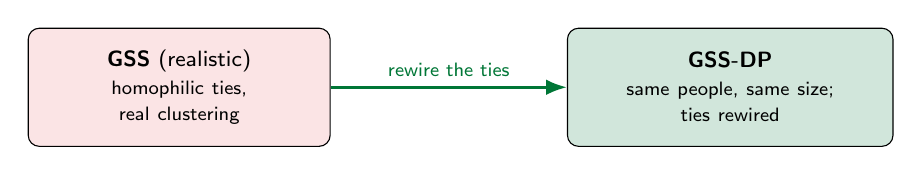
\begin{tikzpicture}[every node/.style={font=\footnotesize,align=center}, node distance=0.7cm]
  \node[draw,rounded corners,fill=ndred!12,text width=3.6cm,minimum height=1.5cm] (gss)
    {\textbf{GSS} (realistic)\\[2pt]\scriptsize homophilic ties,\\ real clustering};
  \node[draw,rounded corners,fill=ndgreen!18,text width=3.9cm,minimum height=1.5cm,right=3.0cm of gss] (rnd)
    {\textbf{GSS-DP}\\[2pt]\scriptsize same people, same size;\\ ties rewired};
  \draw[-{Latex},ndgreen,line width=1pt] (gss.east) -- node[above,font=\scriptsize]{rewire the ties} (rnd.west);
\end{tikzpicture}
\end{center}
\vspace{0.25cm}
\begin{itemize}
  \item Random rewiring creates \emphr{long-range bridges} — classic theory says
        this should \emph{help} diffusion \refn{8}.
  \vspace{0.15cm}
  \item Or, if adoption were just the sum of individual preferences,
rewiring the ties should do nothing...
\end{itemize}
\vspace{0.25cm}
\end{frame}

% ---- 7. Simulation design (adapted from SUNBELT deck)
\begin{frame}{Comprehensive simulation design}
Hybrid social contagion via \texttt{netdiffuseR} \refn{7}, over plausible \emphr{GSS}
vs.\ \emphr{GSS-DP} networks.
\vspace{0.2cm}
\begin{itemize}
  \item \textbf{IUL} ($\Gamma$): 41 levels $[0,1]$. \quad \textbf{MSP} ($h$): 13 levels $[0,1]$.
  \item \textbf{Thresholds} $\tau_i\sim\mathcal{N}(\mu,\sigma)$: $\mu\in\{.3,.4,.5,.6\}$, $\sigma\in\{.08,.12,.16,.20\}$.
  \item \textbf{Seeding}: random, central, marginal, closeness, eigenvector.
\end{itemize}
\vspace{0.2cm}
\begin{center}
Total: $\;41\times13\times4\times4\times5\times \text{(runs)} \;\approx\; \emphr{$4\times10^{6}$ simulations}$
\end{center}
\vspace{0.2cm}
We then fit \emph{Big Additive Models} (BAM) to isolate the structural effect:
\begin{equation*}
  \mathrm{logit}\big[\mathbb{E}(\Phi)\big]=\beta_0+\mathbf{Z}\boldsymbol\beta
  +\beta_{\text{R}}\,\mathbb{I}_{\text{Randomized}}+s(\mathrm{IUL},\mathrm{MSP})
\end{equation*}
\end{frame}

% ================================================================ RESULTS
\sectionslide{Results}

% ---- 8. RESULT 1: adoption maps (copied from SUNBELT deck)
\begin{frame}{Result 1 — The dynamics}
\centering
% crop: keep only the TOP row (Total / Rational / Social adoption); drop the bottom row
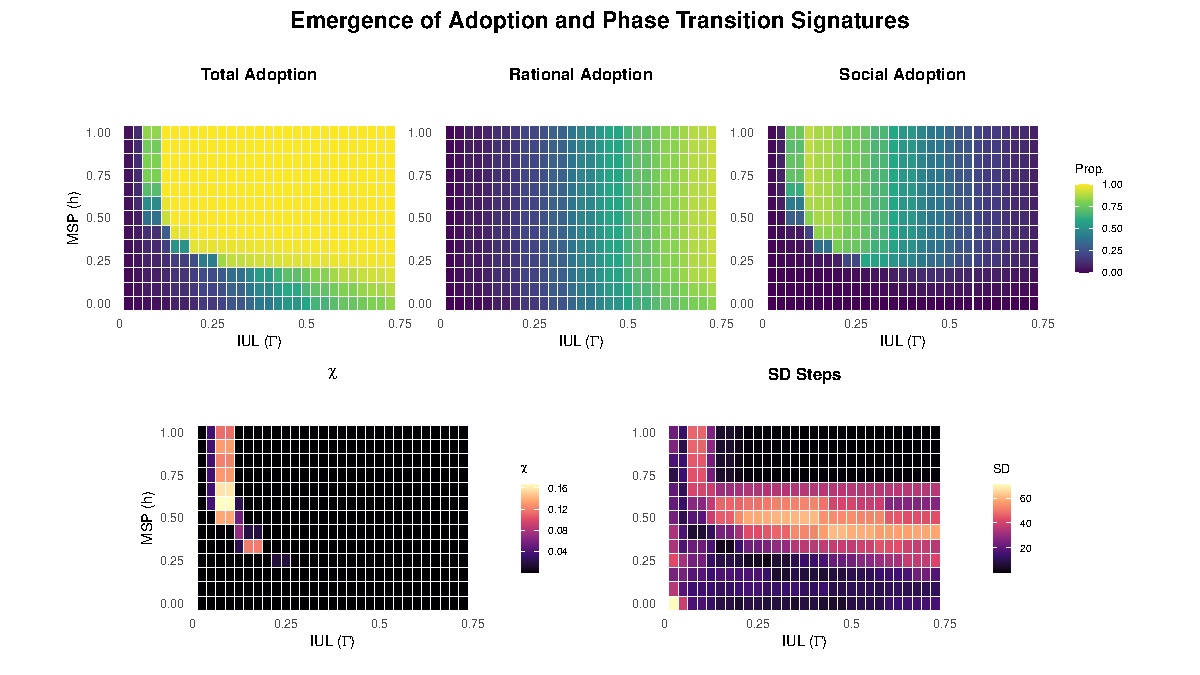
\includegraphics[trim={0 5.25cm 0 1.1cm}, clip, width=1.02\textwidth]{../abstract-sn26/figure1_5panels_GSS.pdf}\\[4pt]
{\footnotesize Mean adoption over the attractiveness (IUL) -- openness (MSP) plane. \\
\emphr{Rational} adoption grows with attractiveness; \emphr{social} adoption is more
complex, so total adoption stays high over a wide region \emph{even when the behavior is
barely attractive}.}
\end{frame}

% ---- 9. RESULT 2: non-structural blocking of complex contagion (GSS only) ----
\begin{frame}{Result 2 — A \emph{non-structural} blocking of complex contagion}
\begin{center}
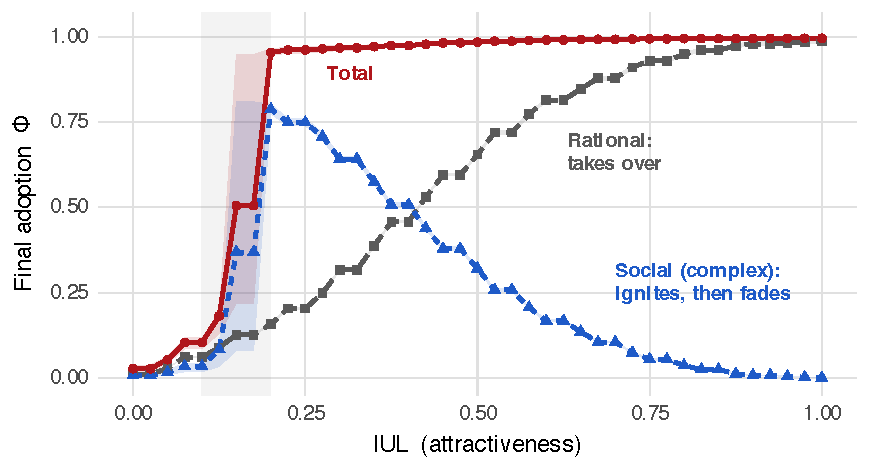
\includegraphics[width=0.62\textwidth]{figure_blocking_gss_eusn.pdf}
\end{center}
\vspace{-0.1cm}
\begin{center}\small
Centola \& Macy \refn{9} already showed a structural barrier to complex diffusion. \\
This is a \emphr{non-structural} blocking of diffusion of collective behavior.
\end{center}
\end{frame}

% ---- 10. RESULT 3: the structural premium + channel split ----
\begin{frame}{Result 3 — What happens when we rewire?}
\begin{columns}[c]
\column{0.5\textwidth}
\small
Same individuals, same preferences.\\
And the \emphr{rewiring created long-range bridges} that should have helped \refn{8,9}.
\begin{itemize}\small
  \item even when we have both Simple and Complex contagion, the bridges are useless.
\end{itemize}
\vspace{0.25cm}
Homophilic \emphr{echo chambers} give social reinforcement and redundancy.
\column{0.47\textwidth}
\centering
\renewcommand{\arraystretch}{1.5}
{\footnotesize
\begin{tabular}{@{}lccc@{}}
\toprule
\textbf{GSS vs GSS-DP} & $\beta$ & OR & odds \\
\midrule
\rowcolor{ndred!10} \textbf{Total adoption} & $-0.850^{***}$ & 0.43 & \emphr{$-57\%$} \\
\rowcolor{ndblue!10} Social adoption & $-0.426^{***}$ & 0.65 & $-35\%$ \\
Rational adoption & $-0.114^{***}$ & 0.89 & $-11\%$ \\
\bottomrule
\end{tabular}}
\\[6pt]
{\scriptsize $^{***}p<0.001$; BAM, ref.\ = GSS; controls: thresholds, seeding,
$s(\mathrm{IUL},\mathrm{MSP})$. Dev.\ expl.\ $\approx83\%$.}
\end{columns}
\end{frame}

% ================================================================ CLOSE
% ---- 11. Conclusions ----
\begin{frame}{Conclusions}
\begin{enumerate}
  \item \textbf{A method:} build \emphr{realistic} whole-networks for survey
        respondents out of \emphr{empirical homophily}.
  \vspace{0.15cm}
  \item \textbf{Three findings:} \\
  \hspace{0.5cm} 1. Social influence can explain adoption even for \emph{low attractive} behaviors. \\
  \hspace{0.5cm} 2. A \emphr{non-structural} blocking of diffusion of collective behavior happens because of the Social Influence channel. \\
  \hspace{0.5cm} 3. Rewiring the ties cuts the \emphr{odds of adoption by $-57\%$}, contrary to expectations.
\end{enumerate}
\vspace{0.3cm}
\begin{center}\small
\emph{Where a behavior ends up is not the sum of individual preferences}\\
it is \emphr{governed by the structure of our real ties.}
\end{center}
\end{frame}

% ---- 12. References ----
\begin{frame}{References}
\footnotesize
\begin{enumerate}\itemsep1.2pt
  \item Goldberg (2021). Associative Diffusion \& the Pitfalls of Structural Reductionism. \emph{ASR} 86(6).
  \item McPherson, Smith-Lovin \& Cook (2001). Birds of a Feather. \emph{Annu. Rev. Sociol.} 27.
  \item Granovetter (1978). Threshold Models of Collective Behavior. \emph{AJS} 83(6). / Valente (1996). \emph{Soc. Networks} 18(1).
  \item Centola (2011). An Experimental Study of Homophily in the Adoption of Health Behavior. \emph{Science} 334.
  \item Smith, McPherson \& Smith-Lovin (2014). Social Distance in the U.S. \emph{ASR} 79(3).
  \item McPherson \& Smith (2019). Network Effects in Blau Space. \emph{Socius} 5.
  \item Vega Yon, Olivera M.\ \& Valente (2025). \texttt{netdiffuseR}. \emph{Zenodo}.
  \item Granovetter (1973). The Strength of Weak Ties. \emph{AJS} 78(6).
  \item Centola \& Macy (2007). Complex Contagions and the Weakness of Long Ties. \emph{AJS} 113(3).
  \item Tur, Zeppini \& Frenken (2024). Diffusion in Small Worlds with Homophily and Social Reinforcement. \emph{Soc. Networks} 76.
  \item Macy \& Evtushenko (2020). Threshold Models of Collective Behavior II. \emph{Sociological Science} 7.
  \item Sethna (2021). \emph{Statistical Mechanics: Entropy, Order Parameters, and Complexity}. Oxford UP.
\end{enumerate}
\end{frame}

% ---- 13. Thanks + QR (copied from SUNBELT deck) ----
\begin{frame}[plain]
  \vfill
  \begin{center}
    {\Large Thanks!}\\[2pt]
    {\color{ndred}\rule{0.30\textwidth}{1.1pt}}\\[0.6cm]
    \qrcode[height=2.2cm]{https://doi.org/10.5281/zenodo.19360209}\\[0.3cm]
    {\footnotesize Scan: preprint draft (Zenodo)}\\[5pt]
    {\footnotesize \texttt{an.oliveram@udd.cl} $\;\cdot\;$ \texttt{aoliveram.cl}}\\[6pt]
    \parbox{0.82\textwidth}{\centering\scriptsize\color{ndgray}
      Olivera Morales, A., Fábrega, J., \& Valente, T. (2026). \emph{Networks Decide for Us:
      Emergence of Adoption in Homophily-Imputed Social Topologies}. Zenodo.
      \texttt{https://doi.org/10.5281/zenodo.19360209}}
  \end{center}
  \vfill
\end{frame}

% ================================================================ BACKUPS
\sectionslide{Backup}

% ---- B1. Which ingredient? (GSS-SH, operational framing) ----
\begin{frame}{Backup — Which ingredient? Scrambling \emph{people}, not ties}
\begin{columns}[c]
\column{0.52\textwidth}
\small
A third network: \emphr{GSS-SH} — keep the graph \emph{byte-identical} (every
triangle, every clique), and \emphr{shuffle who sits where}.\\[4pt]
Your neighbors stay your neighbors in the graph — but they become
\emph{social strangers}: mean social distance on ties jumps $+74\%$.
\vspace{0.3cm}
\begin{center}
\renewcommand{\arraystretch}{1.4}
{\small
\begin{tabular}{@{}lcc@{}}
\toprule
\textbf{vs.\ GSS} & OR & odds drop \\
\midrule
\rowcolor{ndblue!12} GSS-SH (scramble people) & 0.465 & \emphr{$-53\%$} \\
\rowcolor{ndgreen!12} Randomized (rewire ties) & 0.432 & \emphr{$-57\%$} \\
\bottomrule
\end{tabular}}
\end{center}
\column{0.44\textwidth}
\small
Scrambling the people alone reproduces \emphr{$\sim$91\%} of the full penalty:
\emphr{neighbor similarity} carries the premium.
\vspace{0.3cm}

Why not a clean ``topology-only'' cell? Because in these networks
\emphr{clustering emerges from homophily} — re-simulating the homophily-only
ERGM regenerates the triangles. They come as a package:
\emph{clustering is crystallized homophily.}
\\[6pt]
{\scriptsize (3-level BAM; $\beta_{\text{SH}}=-0.766$, $\beta_{\text{R}}=-0.840$;
main-slide 2-level estimates differ negligibly.)}
\end{columns}
\end{frame}

% ---- B2. Physics mapping (copied from CPIN deck) ----
\begin{frame}{Backup — Mapping social adoption to a ferromagnet}
\begin{columns}[c]
\column{0.56\textwidth}
\renewcommand{\arraystretch}{1.35}
\begin{tabular}{@{}l@{\;\;}c@{\;\;}l@{}}
\toprule
\textbf{Ising system} & & \textbf{NDFU} \\
\midrule
Spin $s_i\in\{0,1\}$        & $\leftrightarrow$ & Adoption state $a_i$ \\
Magnetization $M$           & $\leftrightarrow$ & Adoption $\Phi=N_{\text{ad}}/N$ \\
External field $H$          & $\leftrightarrow$ & \emphr{IUL} \\
Temperature $T$             & $\leftrightarrow$ & \emphr{MSP} \\
Exchange $J_{ij}$           & $\leftrightarrow$ & Clustering $w_{ij}$ \\
Susceptibility $\chi$       & $\leftrightarrow$ & $\mathrm{Var}(\Phi)$ \\
\bottomrule
\end{tabular}
\column{0.44\textwidth}
\small
Pseudo-Hamiltonian \refn{12}:
\begin{equation*}
\mathcal{H}\approx -\!\!\sum_{\langle i,j\rangle}\! w_{ij}(h)\,s_i s_j \;-\; \Gamma\sum_i s_i
\end{equation*}
\vspace{0.1cm}
\emphr{Low MSP} $\to$ rigid echo chambers.\\[3pt]
\emphr{High MSP} $\to$ boundaries ``melt''.
\end{columns}
\vspace{0.3cm}
\begin{center}\small
This is why MSP behaves as a social ``temperature''.
\end{center}
\end{frame}

% ---- B2b. The tipping, compared (moved from main deck) ----
\begin{frame}{Backup — The tipping point, compared}
\begin{center}
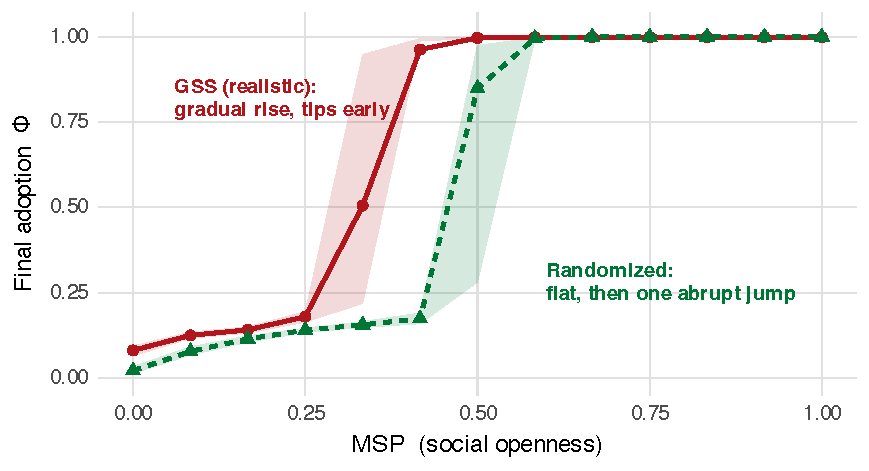
\includegraphics[width=0.66\textwidth]{figure_tipping_cut_eusn.pdf}
\end{center}
\vspace{-0.1cm}
\begin{center}\small
Rewiring the ties also changes the \emph{shape} of the tipping: the realistic network
tips \emphr{earlier and gradually}, through intermediate states;\\
the randomized one stays flat and then jumps in \emphr{one abrupt step} — the
hit-or-flop pattern of Tur et al.\ \refn{10}.
\end{center}
\end{frame}

% ---- B3. The shape of change, quantified ----
\begin{frame}{Backup — The shape of change, quantified}
\small
Near the tipping point, the variance of outcomes diverges as a power law,
$\chi=\mathrm{Var}(\Phi)\sim|MSP-MSP_c|^{-\gamma}$:
\vspace{0.3cm}
\begin{center}
\renewcommand{\arraystretch}{1.2}
{\normalsize
\begin{tabular}{@{}lccc@{}}
\toprule
Susceptibility exponent $\gamma$ (mean) & \textbf{GSS} & \textbf{GSS-SH} & \textbf{Randomized} \\
\midrule
 & $\approx 0.91$ & $\approx 1.08$ & $\approx 3.9$ \\
\bottomrule
\end{tabular}}
\end{center}
\vspace{0.3cm}
\begin{itemize}
  \item GSS and GSS-SH: clean power law, $\gamma\approx1$ — a \emphr{continuous},
        signposted transition (rising variance before the tip).
  \item Randomized: no clean power law — the fit ``$\gamma\approx4$'' is the
        fingerprint of a \emphr{discontinuous}, all-or-nothing jump.
  \item These are ensemble statements (distribution over comparable runs),
        not single-history forecasts.
\end{itemize}
\end{frame}

% ---- B4. Technical details (copied from SUNBELT deck) ----
\begin{frame}{Backup — Technical details}
\begin{itemize}
  \item \textbf{Social distance} $d_{ij}\in[0,1]$ — Gower distance over the Blau-space
        attributes (race, sex, religion, age, education):
\end{itemize}
\begin{equation*}
  d_{ij} = \frac{1}{p}\sum_{k=1}^{p} \delta_{ij}^{k},
  \qquad
  \delta_{ij}^{k} =
  \begin{cases}
    \mathbb{1}\!\left[x_i^{k}\neq x_j^{k}\right] & \text{categorical } (\text{race, sex, religion})\\[4pt]
    \dfrac{\big|x_i^{k}-x_j^{k}\big|}{\max_k - \min_k} & \text{numeric } (\text{age, education})
  \end{cases}
\end{equation*}
\vspace{0.3cm}
\footnotesize
* The idiosyncrasy that drives adoption of barely-attractive behaviors here is
\emphr{measured preference} and \emphr{realistic structure}, not stochastic noise
(Macy \& Evtushenko \refn{11}).
\end{frame}

\end{document}
